%\documentclass[fullpage,fleqn,leqno]{article}

\documentclass[twoside]{article}%{combine}
%\usepackage{url}
\usepackage{../../tex/html}
\usepackage{amsfonts,amsmath,color,amsthm,amssymb, enumerate, bbm, subfig}
\usepackage{graphicx}
%\usepackage[DIV=14,BCOR=2mm,headinclude=true,footinclude=false]{typearea}
%\usepackage[font=small,labelfont=bf]{caption}
\usepackage{hyperref}
\usepackage{tikz, etoolbox}

\usetikzlibrary{shapes}
\usetikzlibrary{arrows}
%\usepackage[margin=1in]{geometry}
\usepackage{graphicx,amsmath,gentium,tikz,caption}
\usetikzlibrary{patterns}
\usetikzlibrary{matrix,arrows,positioning,shapes}
\usetikzlibrary{arrows.meta}
\tikzset{
  a/.style={-{Stealth[scale=1.3,angle'=45]},semithick}
}
%\usepackage{xfrac,fontspec,unicode-math}
%\setmathfont[version=cambria]{Cambria Math}
%\mathversion{cambria}
\usepackage[letterpaper, portrait, margin=1.1in]{geometry}
\usepackage{amsmath,amsthm}
\usepackage{mathtools}
\newtheorem*{definition}{Definition}
\usepackage{tcolorbox}
\tcbset{colback=white,colframe=black}
\everymath{\displaystyle}

\makeatletter
\@ifundefined{namelength}{
\newlength{\namelength}
\settowidth{\namelength}{{\bf \Large Name: }}
\newlength{\namelinelength}
\setlength{\namelinelength}{\textwidth}
\addtolength{\namelinelength}{-\namelength}
}{}

\@ifundefined{vs}{
\newcommand*{\vs}[1]{\par
  \vspace*{#1\baselineskip}%
  \@afterindentfalse
  \@afterheading
}
}{}
\makeatother



\def\fancytitle#1#2#3{
      \centerline{\framebox{\framebox{ \parbox{.8\textwidth}{ \bf ENGRI 1101 \hfill
      Engineering Applications of OR \ \ \ \  Fall 2020 \hfill #3 #1 \\
\mbox{ }\hfill
      \hfill\mbox{ } \\[1mm] \mbox{ } \hfill{\Large \bf #2}\hfill
      \mbox{ }} }}}
      
\vs 2
}

\def\handout#1#2{\fancytitle{#1}{#2}{Handout}}
\def\review#1#2{\fancytitle{#1}{#2}{Review}}
\def\homework#1#2{\fancytitle{#1}{#2}{Homework}}
\def\exercises#1{\fancytitle{}{#1}{Exercises}}
\def\solution#1#2{\fancytitle{#1}{#2}{Solutions}}
\def\final#1#2{\fancytitle{#1}{#2}{Final}
      \noindent {\bf \Large Name:} \rule{\namelinelength}{0.5pt}
      \vspace*{\baselineskip}}
\def\prelim#1#2{\fancytitle{#1}{#2}{Prelim}
      \noindent {\bf \Large Name:} \rule{\namelinelength}{0.5pt}
      \vspace*{\baselineskip}}
\def\quiz#1#2{\fancytitle{#1}{#2}{Quiz}
      \noindent {\bf \Large Name:} \rule{\namelinelength}{0.5pt}
      \vspace*{\baselineskip}}
\def\lab#1#2{\fancytitle{#1}{#2}{Lab}
      \noindent {\bf \Large Name:} \rule{\namelinelength}{0.5pt}
      \vspace*{\baselineskip}}
\def\prelab#1#2{\fancytitle{#1}{#2}{Prelab}
      \noindent {\bf \Large Name:} \rule{\namelinelength}{0.5pt}
      \vspace*{\baselineskip}}

\raggedbottom









%\usepackage{html}
%\usepackage{fullpage}
%\usepackage{enumitem}
%\usepackage{amsfonts,amsmath,color,amsthm,amssymb, enumerate, bbm, subfig, hyperref}
%\usepackage[normalem]{ulem}
%\usepackage{graphicx}
%\newcommand{\vs}[1]{\vspace{#1 pt}}

\definecolor{purple}{RGB}{128,0,128}
\newcommand{\com}[1]{{\bf {\color{red} #1}}}

%\usepackage{graphicx,amsmath,gentium,tikz,caption}
\usetikzlibrary{patterns}
\usetikzlibrary{matrix,arrows,positioning,shapes}
\usetikzlibrary{arrows.meta}
\tikzset{
  a/.style={-{Stealth[scale=1.3,angle'=45]},semithick}
}
%\usepackage{xfrac,fontspec,unicode-math}
%\setmathfont[version=cambria]{Cambria Math}
%\mathversion{cambria}
\usepackage[letterpaper, portrait, margin=1.1in]{geometry}
\usepackage{amsmath,amsthm}
\usepackage{mathtools}
\newtheorem*{definition}{Definition}
\usepackage{tcolorbox}
\tcbset{colback=white,colframe=black}
\everymath{\displaystyle}

\makeatletter
\@ifundefined{namelength}{
\newlength{\namelength}
\settowidth{\namelength}{{\bf \Large Name: }}
\newlength{\namelinelength}
\setlength{\namelinelength}{\textwidth}
\addtolength{\namelinelength}{-\namelength}
}{}

\@ifundefined{vs}{
\newcommand*{\vs}[1]{\par
  \vspace*{#1\baselineskip}%
  \@afterindentfalse
  \@afterheading
}
}{}
\makeatother



\def\fancytitle#1#2#3{
      \centerline{\framebox{\framebox{ \parbox{.8\textwidth}{ \bf ENGRI 1101 \hfill
      Engineering Applications of OR \ \ \ \  Fall 2020 \hfill #3 #1 \\
\mbox{ }\hfill
      \hfill\mbox{ } \\[1mm] \mbox{ } \hfill{\Large \bf #2}\hfill
      \mbox{ }} }}}
      
\vs 2
}

\def\handout#1#2{\fancytitle{#1}{#2}{Handout}}
\def\review#1#2{\fancytitle{#1}{#2}{Review}}
\def\homework#1#2{\fancytitle{#1}{#2}{Homework}}
\def\exercises#1{\fancytitle{}{#1}{Exercises}}
\def\solution#1#2{\fancytitle{#1}{#2}{Solutions}}
\def\final#1#2{\fancytitle{#1}{#2}{Final}
      \noindent {\bf \Large Name:} \rule{\namelinelength}{0.5pt}
      \vspace*{\baselineskip}}
\def\prelim#1#2{\fancytitle{#1}{#2}{Prelim}
      \noindent {\bf \Large Name:} \rule{\namelinelength}{0.5pt}
      \vspace*{\baselineskip}}
\def\quiz#1#2{\fancytitle{#1}{#2}{Quiz}
      \noindent {\bf \Large Name:} \rule{\namelinelength}{0.5pt}
      \vspace*{\baselineskip}}
\def\lab#1#2{\fancytitle{#1}{#2}{Lab}
      \noindent {\bf \Large Name:} \rule{\namelinelength}{0.5pt}
      \vspace*{\baselineskip}}
\def\prelab#1#2{\fancytitle{#1}{#2}{Prelab}
      \noindent {\bf \Large Name:} \rule{\namelinelength}{0.5pt}
      \vspace*{\baselineskip}}


\begin{document}

\lab{2}{The Shortest Path Problem}

\noindent
\subsection*{Objectives}
\begin{itemize}
\item   Introduce students to the concept of a shortest path tree
\item   Show students the inner workings of a combinatorial algorithm
\item   Demonstrate the usefulness of sensitivity analysis in problem solving
\end{itemize}

\subsection*{Optional Reading Assignment}
\begin{itemize}
\item
Read Handout 3 on the shortest path problem.
\end{itemize}

\vs 2

\subsection*{Brief description}
In this lab, we review some motivation and observations behind Dijkstra's algorithm for shortest path computation, and analyze how sensitive the solution to the shortest path problem is to changes in the input data.

\newpage

\subsection*{Part \#1: The shortest path problem, and Dijkstra's algorithm}

As an Entrepreneurial first-year student, you plan to start a pizza delivery company: Good Pizza, Inc.  You will base Good Pizza out of the kitchen on your floor of Jameson Hall and deliver pizzas via bike.  You want to guarantee delivery anywhere on campus in 15 minutes or less; in order to maximize the amount of your tips, you want to deliver as many pizzas as you can and deliver
them as fast as you can.  As a first-year, however, you're still figuring out your way around campus.  You've quickly realized that, because of pedestrian traffic, lights, obstacles, and  placement of bike stands  it is not always best to take the route that covers the shortest distance.  Instead, you would like to know the
quickest way of getting from the your dorm room to various parts of campus.

To help you in finding the quickest routes, you map the travel time between some of the most-happening locations on campus.  Below is an attached map showing the key points on campus.  There are several copies of this graph at the end of the lab, which may be useful throughout. 

\begin{center}
\includegraphics[width=0.8 \textwidth]{campusmap.png}
\end{center}

The next page shows a stylized graph of the map above indicating travel times. Note that the positions of some nodes have been slightly modified on the graph so that it is easier to view the information.

\newpage

\begin{center}
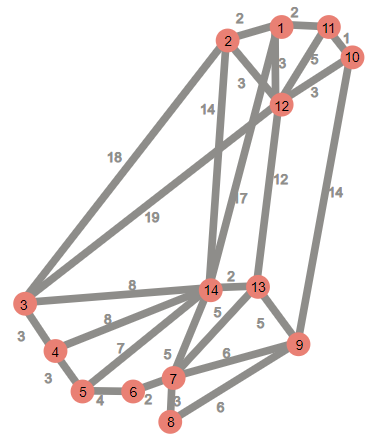
\includegraphics[width=0.5\textwidth]{Graph.png}
\end{center}

\bigskip

\noindent

Let's load up this graph!  Go to \url{http://engri1101.orie.cornell.edu/} and click \texttt{Dijkstra's Shortest Path}. You should see a digital copy of the above graph, and tables set up to run Dijkstra's algorithm.  

\noindent
Your company is based out of Jameson Hall, which is node $1$.  We'll treat this node as our source $s$. 

What is the node that is closest to  Jameson Hall (not considering  Jameson Hall itself)? In case of ties, choose any of them.
Can there be a quicker route to get to this destination (call it point
$X$) than just to go directly there from  Jameson Hall? Why or why not?

\vskip .7in

\noindent
Explain why the predecessor (``prev$(X)$'' from class) of $X$ must be the  Jameson Hall.

\vskip 1in

\noindent
For now on, let $X$ be High Rise 5 ($X$ has ID 11).  On the web app, first click the node labelled 1 to start running Dijkstra's algorithm.  Then select node 11. 

After clicking those two nodes, you should notice that several things happen:
\begin{itemize} 
\item Node 1 and 11 turn solid blue, and the edge between them darkens; this edge has been ``added to the shortest path tree.''
\item  The tables on the right update, and you can see the current version of the Dijkstra table (iteration 2).  You can also compare this to the previous table (for iteration 1), faded out below it.
\item In the current table, node 11 is now starred and prev(11) is marked as node 1.
\end{itemize}

\noindent
The graph shows styles of nodes:
\begin{itemize}
\item Fully blue nodes (1 and 11)
\item Fully red nodes (e.g. nodes 3 and 9)
\item Red nodes with a blue perimeter (e.g. nodes 2 and 14).
\end{itemize}
What does each style of node represent?

\vskip 1in



 How do we find the next edge to add to the tree (i.e., the next edge to ``darken'')?
One way is as follows. Compute the travel times for all routes that
either go directly from  Jameson Hall to a destination or go from  Jameson Hall to
point $11$ and then directly to a destination. Take the shortest of all
these routes and add it to the tree. For instance, in this case, we
consider the following routes. Node IDs are in parenthesis.

\smallskip

\begin{tabular}{ll}
\underline{Route}   &\underline{Travel Time}\\
 Jameson Hall (1) - High Rise 5 (11) & {\bf 2} \\
 Jameson Hall (1) - Clara Dickson Hall (2) & 2* \\
 Jameson Hall (1) -  Helen Newman (12)  &  3\\
 Jameson Hall (1) - Lynah Hockey Rink  (14)   &17 \\
Jameson Hall (1) - High Rise 5 (11) - Holland International Living Center (10)  &3  \\
Jameson Hall (1) - High Rise 5 (11) - Helen Newman  (12)  & 7 \\
\end{tabular}

Consider all of the nodes we can reach by these paths (e.g. 1, 11, 2, 12, 14, and 10).  What is true about those nodes -- and only those nodes -- in the web-app table for iteration 2?  

\vskip .7in


\noindent There are two paths to node 12 listed above.  Look at node 12 in the table for iteration 2.  Which of those two paths is indicated in the table?  Using just the table -- without referring back to the original graph or edge lengths -- how can you identify this path?

\vskip .7in


\noindent
Now back to Dijkstra and we pick Clara Dickson.  Jameson Hall to Clara Dickson is the shortest route on this list (we've marked it
with a *). Can there be a shorter route to Clara Dickson than the one that we just added? Why
or why not?  Answer this question in as much generality as possible.  Hint: suppose that there were some shorter path that went from Jameson -- SOMEWHERE ELSE -- Clara Dickson.  How would the length of the first edge in this path have to compare to the length of the edge directly between Jameson and Clara Dickson?

\vskip .7in

\noindent
Now we update the table for the next iteration: if two entries have the same destination we
drop the more expensive one (e.g., we drop the Jameson Hall - High Rise 5 - Helen Newman route, since we it takes longer than the direct Jameson Hall - Helen Newman route).
Then for each destination that can be reached from Clara Dickson, we compute
the length of the path using only nodes already marked, with
Clara Dickson being the second-to-last node on the path. Fill in the missing
entries in the table below.  Then, as before, cross out any redundant paths (like the Jameson Hall - High Rise 5 - Helen Newman path which we previously dropped).

\medskip

\begin{tabular}{ll}
\underline{Route}       &\underline{Travel Time}\\
 Jameson Hall (1) - High Rise 5 (11) & {\bf 2} \\
 Jameson Hall (1) - Clara Dickson Hall (2) & {\bf 2} \\
 Jameson Hall (1) -  Helen Newman (12)  &  3\\
 Jameson Hall (1) - Lynah Hockey Rink  (14)   &17 \\
Jameson Hall (1) - High Rise 5 (11) - Holland International Living Center (10)  &3  \\
 Jameson Hall (1) - Clara Dickson Hall (2) - ... & ... \\
 Jameson Hall (1) - Clara Dickson Hall (2) - ... & ... \\
 Jameson Hall (1) - Clara Dickson Hall (2) - ... & ... \\
\end{tabular}


\medskip
\noindent
On the web app, click node 2 (when we click node 2, we ``mark it.''  This marking is encoded in the graph when the corresponding node turns blue, and with a * in the updated table for iteration 3).  Use the updated table for iteration 3 to verify your work.

\medskip
\noindent
Choose the next edge to be added to the
shortest path tree.  List both the next node to click and the corresponding edge that will be darkened.

\vskip 1in


\noindent
Dijkstra's Algorithm continues in this manner. In the next step, we
compute the travel times to destinations not already marked (i.e. starred/fully blue) that
are adjacent to the lastly marked node, using routes that involve only
already marked nodes as intermediate steps.
Do the next iteration of the algorithm by hand based on your previous answer: write down the nodes
that get marked and/or have their labels updated in this iteration.  It will help to look at the map attached to the end of this lab (you can rip off the last page and use it as a reference throughout the lab).

\vskip 2.5in

\noindent

Now trace the execution of Dijkstra's algorithm with the software
up to the point that you have already computed by hand: at each step, click the next node to mark on the software.  You should be able to readily identify this node based off the table shown on the web app.

\vskip 1in

\noindent
Now highlight the shortest path tree you just found on the copy of the map at the end of this packet. How
can you read out the shortest path from  Jameson Hall to other places in
on campus from the shortest path tree? 


\vskip 1in

\noindent What is the shortest path (both the route and length) from  Jameson Hall to Rhodes Hall (node 8)?

\vskip .8in

\noindent
Is the 15 minute guarantee a good one? What about a 30 minute guarantee, assuming some reasonably small fluctuations in the actual travel time due to traffic, etc.
\vskip .8in

\noindent
Is the shortest path always unique? If yes, why? If no, can you give
an example of two nodes in the graph for this lab that have more than
one shortest path between them?

\vskip .8in


\noindent
\subsection*{Part \#2: Sensitivity analysis}


\smallskip

\noindent
The next several questions ask you to analyze how sensitive your
output is to the precise data that has been used. This is called
``performing sensitivity analysis'' for the input.

\smallskip

\noindent
Suppose that there was a parade on campus so that the time
to go from Holland International (10) to Cornell High Energy (9) {\it directly} was increased to 20 minutes.

 Would this change
the shortest path tree? How would the shortest path tree change?  

\vskip 1.5in


\noindent
Can such an increase affect any of the routes that did not originally
include the leg from Holland International (10) to Cornell High Energy (9)? Why or why not?

\vskip 1.5in

\noindent Now verify your answers!  Click the ``double arrow'' button below the graph (the button on the left, with two arrows in different directions).  This feature will allow you to change the length of an edge: on the first prompt enter 10, on the second prompt enter 9, and on the third prompt enter 20.  The edge between nodes 9 and 10 should now have cost 20.  Rerun Dijkstra's algorithm (feel free to click the fast forward button).  Did you make any mistakes?

\vskip 1.5in

\noindent
Suppose that travel time from node (10) to node (9) increased from 14 minutes, but not all the way to 20 minutes.  By how much could the travel time increase {\bf without} the shortest path route to node (9) changing (i.e. matching the original route found by the web app)?


\vskip 1.5in

\noindent
Hit the reset (circular arrow) button below the graph.  Doing so resets any changes to the original edge lengths.  Suppose that your competitor, Better-Than-Adequate Pizza, decides to promote their brand by installing a moving walkway that takes students from Clara Dickson on North Campus to the Lynah hockey rink.  This has the effect of reducing the travel time from Clara Dickson (2) to Lynah (14) so that it only takes 5 minutes.  Would this change alter the shortest path tree? Does this
affect any of the routes that did not originally include the
leg from Clara Dickson to Lynah? Why or why not?  Feel free to check your work by asking the program to change the length of the edge between nodes 2 and 14.

\vskip 1.5in

\noindent
Suppose that all the travel times obeyed the following inequality:
\begin{center}
(travel time from A to C) $\le$ (travel time from A to B) + (travel
time from B to C)
\end{center}
for all nodes $A$, $B$ and $C$.  This is called the {\bf triangle
inequality}. Suppose our input was the complete graph (that is, there is an edge between every pair of nodes).  If the travel times on this input obeyed the triangle inequality, what would the shortest path tree look like?

\vskip 1.5in

\noindent
\subsection*{Part \#3: NYC Data}


\smallskip

\noindent
Download the entire folder Lab 2 Extension from Canvas. Open the .ipynb file in Jupyter notebook, and work through the Juypter notebook.  Then, answer the following questions after going through the NYC pizza example.

\smallskip

\noindent
What is the variable \textit{dfl}, and what are its columns?

\vskip 0.9in

\noindent
Without a traffic jam on Queensboro Bridge, is a 30-minute guarantee reasonable?

\vskip 0.9in

\noindent
What would you recommend as a delivery time guarantee to all the marked locations given that there are often traffic jams on Queensboro Bridge?

\vskip 0.9in

\newpage
\clearpage

\newpage
\includegraphics[angle=90,width=\textwidth]{campusmap.png}
\newpage
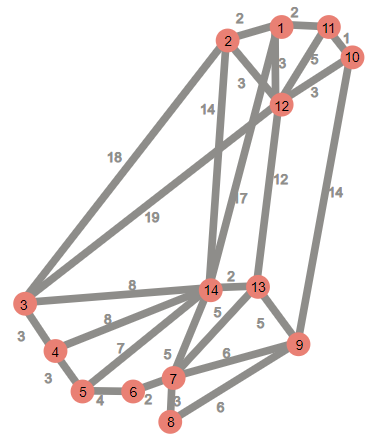
\includegraphics[width=0.8\textwidth]{Graph.png}
\newpage

\end{document}